\documentclass{article}
\usepackage[T1]{fontenc}

\usepackage{graphicx}
\usepackage{parskip}
\usepackage[colorlinks=true,linkcolor=black]{hyperref}
\usepackage[french]{babel}
\usepackage{subcaption}
\usepackage[french]{babel}

\usepackage[margin=3.5cm]{geometry}


\author{Erwan LEMATTRE, Yannis CHUPIN}
\title{Rapport mi-projet\\Fairness pour l'IA}

\begin{document}
    \maketitle
    \newpage
    \tableofcontents
    \newpage

    \section{Introduction}
    Ce projet a pour objectif d'analyser les accidents de la circulation routière afin de pouvoir déterminer 
    à partir des données d'un véhicule accidenté si l'accident est mortel ou non.
    Les données sont des données libres mises à disposition par le \textit{Ministère de l'Intérieur et des 
    Outre-Mer}. Le jeu de données correspond aux accidents de 2005 à 2022 en France. Nous allons, dans une première 
    partie, analyser ces données afin d'extraire les informations utiles à l'apprentissage et de pouvoir repérer 
    d'éventuelles sources de biais pour notre modèle.
    
    Vous pouvez retrouver le code sur le GitHub du projet. Le fichier \texttt{main.ipynb} contient 
    le code principal que nous allons suivre tout au long de ce rapport. Le fichier \texttt{utils.py} 
    contient toutes les fonctions auxiliaires que nous utilisons dans le fichier principal.

    \section{Découverte du jeu de données}
    \subsection{La base de données}
    La base de données est composée de plusieurs tables : \textit{usagers}, \textit{véhicules}, \textit{lieux} et 
    \textit{caractéristiques}. Nous avons joint ces quatre parties pour obtenir un dataframe contenant une 
    cinquantaine de colonnes. 
    On peut retrouver l'ensemble des attributs dans l'annexe \ref{appendix:dataset}.


    \subsection{Répartition des données}
    Afin de pouvoir conserver les données utiles pour l'apprentissage, nous avons analysé la répartition des 
    différentes données dans notre dataframe.
    Nous avons ainsi pu faire différentes observations. 
    \\
    Voici quelques-unes d'entre elles qui nous sont ensuite
    utiles pour la préparation des données.
    \subsubsection{Catégories de véhicule}
    La base de données nous donne beaucoup de catégories différentes. Nous avons cependant pu remarquer 
    que la majorité des véhicules sont dans seulement 5 catégories.
    \begin{figure}[ht]
        \centering
        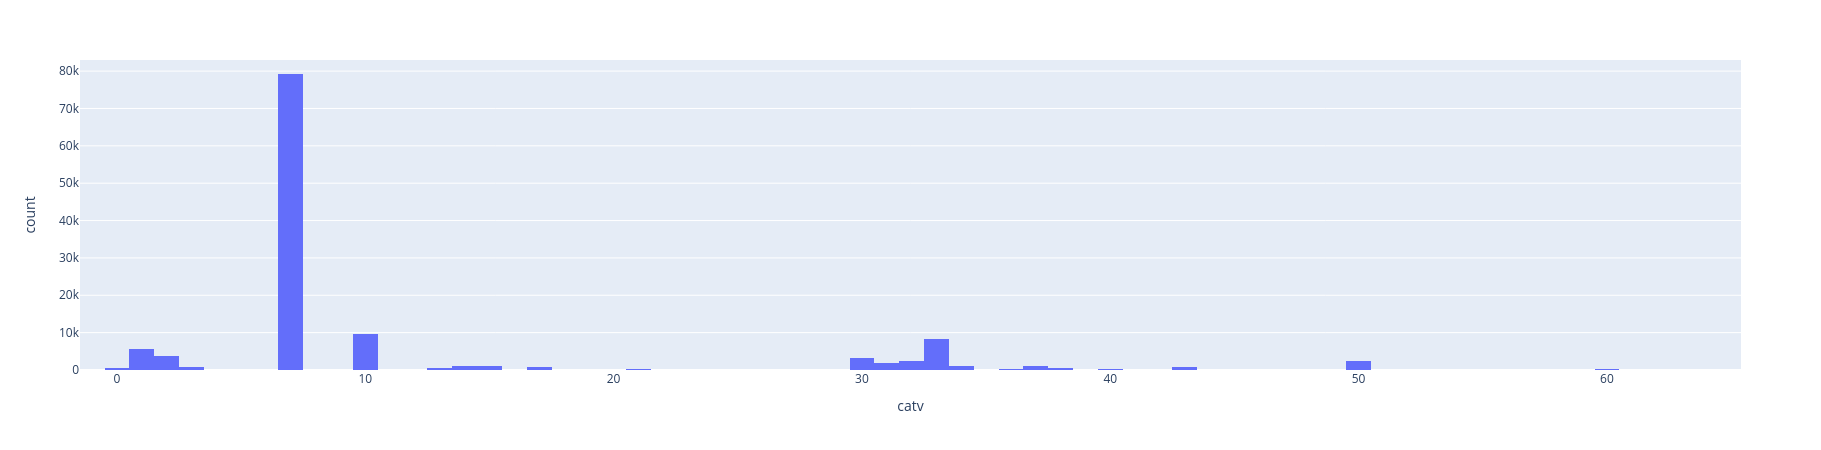
\includegraphics[width=12cm]{./img/catv1.png}
        \caption{Répartition des catégories de véhicules}
    \end{figure}

    \subsubsection{Gravité de l'accident}
    En affichant l'effectif d'accidents mortels, nous avons pu remarquer qu'ils ne représentent qu'une 
    infime partie des accidents. Le peu de données sur ces accidents ne nous permet pas d'apprendre 
    un modèle. C'est la raison pour laquelle nous avons décidé de nous intéresser non pas à la mortalité 
    à l'échelle d'une personne, mais plutôt à l'échelle d'un accident. Nous nous mettons pour cela au niveau d'un 
    véhicule car cela nous permet de conserver plus d'informations (à l'échelle d'un accident, on aurait 
    dû enlever trop d'informations pour ne conserver que les attributs plus généraux à l'accident).

    \begin{figure}[ht]
        \centering
        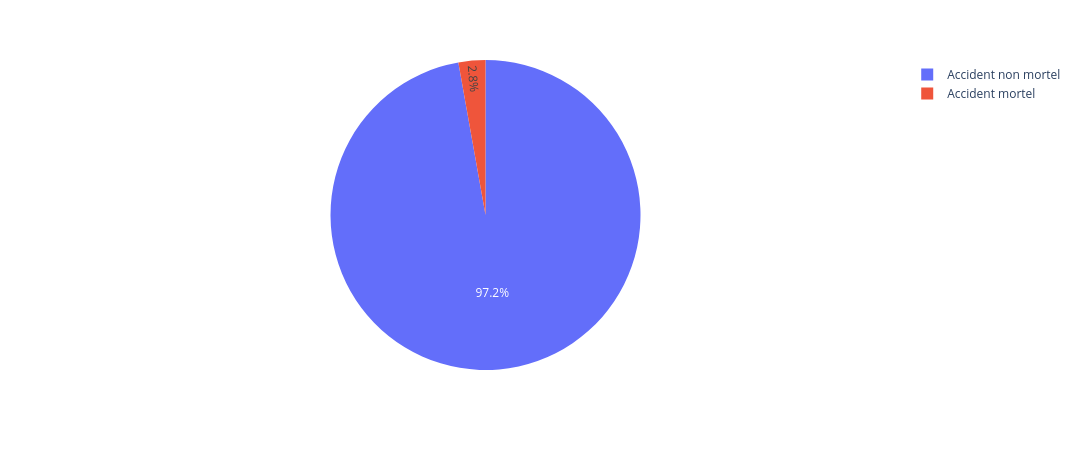
\includegraphics[width=12cm]{./img/grav1.png}
        \caption{Proportion d'accidents mortels}
    \end{figure}

    \section{Préparation des données}
    À partir des observations précédentes, nous avons supprimé les attributs moins intéressants pour l'apprentissage 
    et nous avons modifié certains attributs afin d'en extraire les informations intéressantes.
    \\
    Les attributs supprimés sont : \textit{voie}, \textit{v1}, \textit{v2}, \textit{pr}, \textit{pr1}, \textit{lartpc},
    \textit{larrout}, \textit{num\_veh}, \textit{occutc}, \textit{adr}, \textit{senc}, \textit{etatp}, \textit{actp}, 
    \textit{manv}, \textit{jour}, \textit{com}, \textit{hrmn}, \textit{motor}, \textit{place}, \textit{vosp}, \textit{locp}.
    \\\\
    Nous avons effectué les modifications suivantes :
    \begin{itemize}
        \item Création d'un attribut \textit{mortal} qui vaut 1 si le véhicule est impliqué dans un accident mortel, 0 sinon.
        \item À partir de l'attribut \textit{sexe}, nous avons créé un attribut \textit{sexe\_conducteur} qui garde seulement 
                le sexe du conducteur du véhicule.
        \item Création d'un attribut \textit{piéton} qui vaut 1 si un piéton est impliqué dans l'accident, sinon 0.
        \item Nous avons utilisé l'année de naissance et l'année de l'accident pour récupérer l'âge du conducteur.
        \item L'attribut \textit{vma} a été découpé en 4 catégories de vitesse.
        \item Pour les attributs \textit{catv} et \textit{vatr}, nous avons gardé les valeurs les plus représentées dans la base de données.
    \end{itemize}
    \vspace{0.5cm}
    Nous avons également réduit les valeurs de certains attributs. Par exemple, pour des attributs 
    avec des valeurs telles que \textit{Non-renseigné}, \textit{Autre}, \dots \, nous avons regroupé 
    ces valeurs en une seule valeur. L'objectif était ici de simplifier en réduisant les catégories 
    mais également d'améliorer les performances de notre modèle.

    \section{Analyse des données}
    Une fois nos données préparées, nous avons pu les visualiser. Nous allons montrer dans les 
    deux prochaines parties les observations intéressantes que nous avons pu faire lors de 
    l'analyse de notre dataset.
    
    \subsection{Analyse univariée des données}
    \subsubsection{Les accidents mortels}
    Une donnée intéressante à observer est la proportion de véhicules impliqués dans un accident 
    mortel. C'est en effet la valeur que nous voulons prédire.

    \begin{figure}[ht]
        \centering
        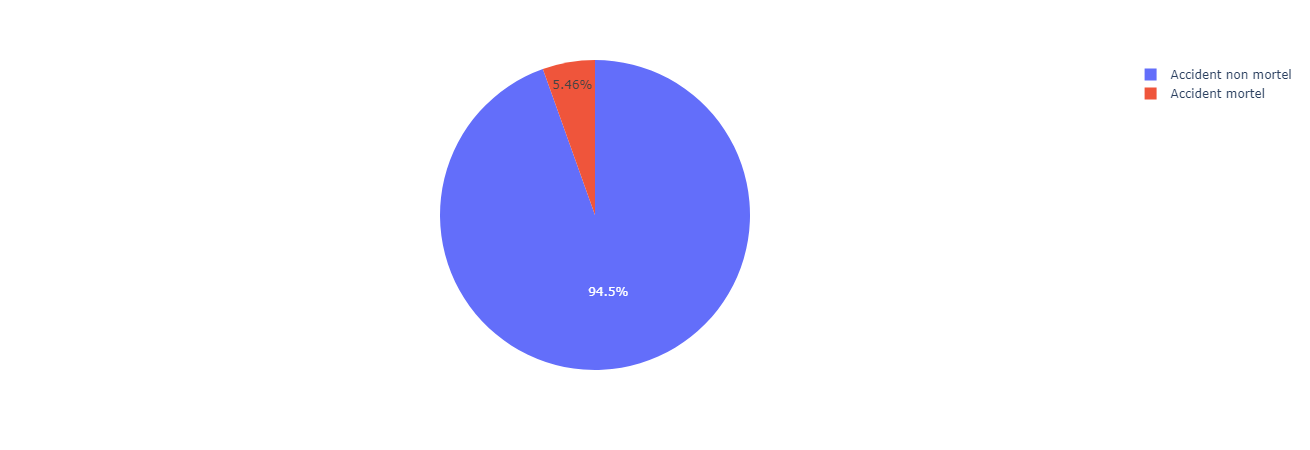
\includegraphics[width=10cm]{./img/grav2.png}
        \caption{Proportion des véhicules impliqués dans un accident mortel}\label{fig:fig_acc_mortel}
    \end{figure}

    Nous pouvons remarquer sur la figure \ref{fig:fig_acc_mortel} que le fait de s'intéresser 
    aux véhicules impliqués dans un accident mortel et non plus aux personnes victimes permet 
    de doubler le pourcentage. Même si cette proportion reste faible, cela va nous permettre 
    d'avoir plus de données dans la catégorie mortelle lors de l'apprentissage et par conséquent 
    d'avoir un meilleur modèle.

    \subsubsection{Les piétons}
    Nous nous sommes ensuite intéressés aux accidents dans lesquels un piéton est impliqué. 
    La figure \ref{fig:fig_acc_pieton} nous montre qu'un peu moins de 10\% des accidents impliquent 
    un piéton.

    \begin{figure}[ht]
        \centering
        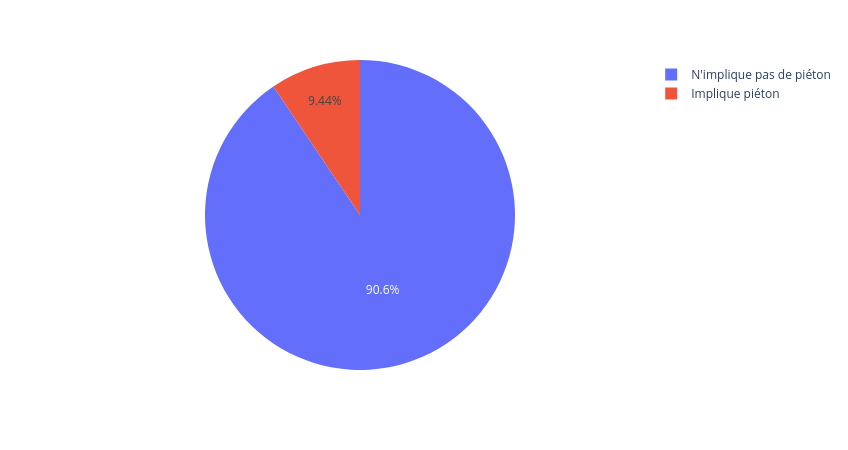
\includegraphics[width=10cm]{./img/pieton.png}
        \caption{Proportion des accidents avec piéton}\label{fig:fig_acc_pieton}
    \end{figure}

    \subsubsection{L'âge}
    Nous pouvons visualiser l'âge des conducteurs via une boîte à moustache. La figure \ref{fig:fig_age} nous 
    montre la répartition de l'âge des conducteurs. Lors du prétraitement des données, les valeurs aberrantes 
    ont été enlevées. On retrouve donc logiquement des âges contenus entre 0 et 100 ans. L'âge médian des 
    conducteurs est 33 ans avec le premier quartile à 21 et le troisième quartile à 49 ans. Même si on peut 
    imaginer que des valeurs sont fausses (il y a des conducteurs de moins de 16 ans), les valeurs sont tout de 
    même assez cohérentes par rapport à ce que l'on pourrait imaginer de la répartition de l'âge des conducteurs.

    \begin{figure}[ht]
        \centering
        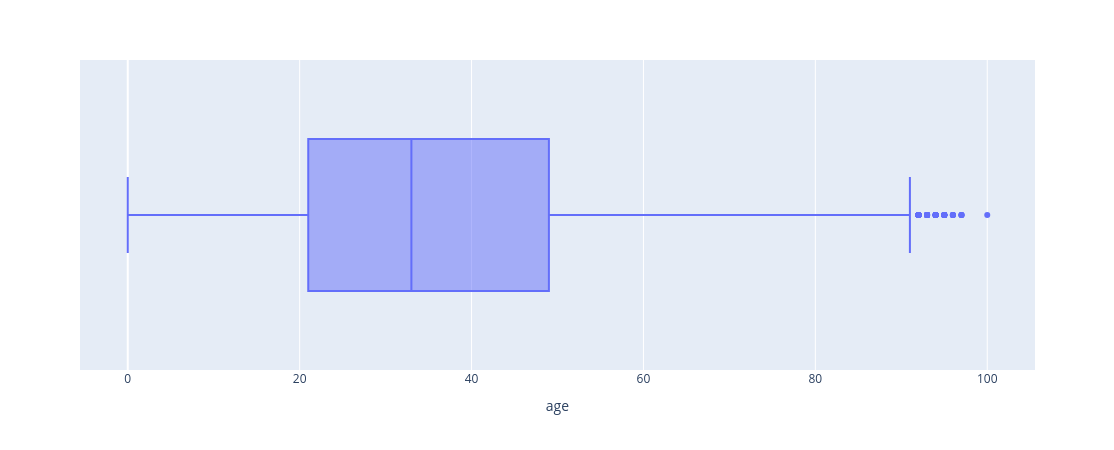
\includegraphics[width=12cm]{./img/age.png}
        \caption{Âge des conducteurs}\label{fig:fig_age}
    \end{figure}

    \subsubsection{Le genre des conducteurs}
    Le genre des conducteurs est assez intéressant à analyser. Sur la figure \ref{fig:fig_genre}, nous pouvons 
    remarquer une différence importante entre le nombre de femmes au volant (indice 0) et le nombre d'hommes au volant 
    (indice 1). Cette différence pourrait être une source de biais pour notre modèle. En effet, le fait qu'il y ait 
    beaucoup plus de données d'accident avec des hommes ne signifie pas qu'il y a plus de chances d'avoir un accident 
    si on est un homme. Cela signifie peut-être que la proportion d'hommes au volant est plus élevée et donc qu'il 
    y a plus d'accidents avec un homme au volant car il y a plus d'hommes au volant. Le risque ici est que notre 
    modèle associe un homme à un accident mortel car il y a beaucoup plus d'accidents mortels avec un homme au 
    volant.

    \begin{figure}[ht]
        \centering
        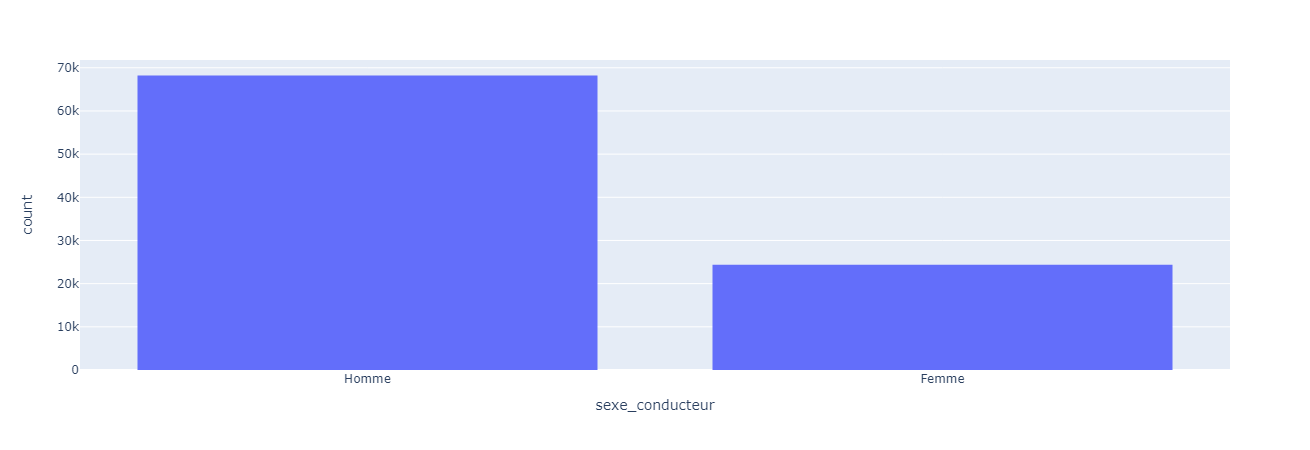
\includegraphics[width=12cm]{./img/sexe.png}
        \caption{Genre des conducteurs}\label{fig:fig_genre}
    \end{figure}

    \subsubsection{Le type de collision}
    La figure \ref{fig:fig_col} montre la répartition des différents types de collisions dans notre dataset. On peut 
    remarquer que tous les types de collisions sont plutôt bien représentés dans notre dataset. C'est un attribut qui 
    pourra être assez intéressant pour l'apprentissage.

    \begin{figure}[ht]
        \centering
        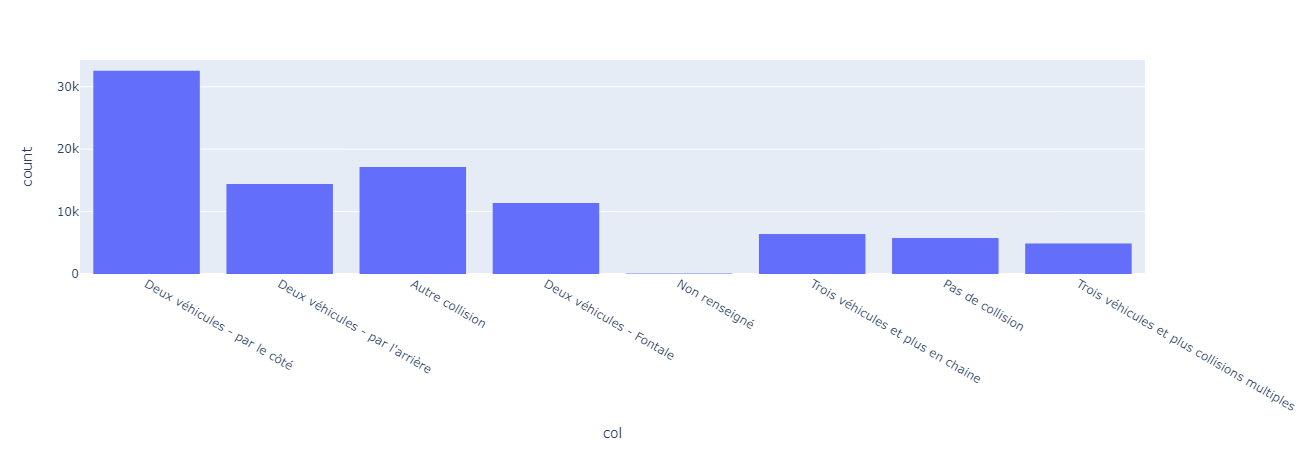
\includegraphics[width=12cm]{./img/col.png}
        \caption{Les types de collision}\label{fig:fig_col}
    \end{figure}

    \subsection{Analyse bivariée des données}
    Nous allons dans cette partie donner quelques exemples intéressants obtenus lors de l'analyse bivariée. On 
    peut retrouver l'ensemble des graphiques observés dans le fichier \texttt{main.ipynb}.

    \subsubsection{Le genre du conducteur}
    Un attribut qu'il est intéressant d'analyser est le genre du conducteur. En effet, il peut être source de biais 
    s'il y a un déséquilibre entre hommes et femmes.
    On retrouve globalement la même proportion dans la corrélation que l'on soit homme ou femme. Les hommes étant 
    beaucoup plus représentés dans le dataset, la proportion d'hommes est logiquement plus élevée. On peut cependant 
    faire quelques remarques. 
    
    La figure \ref{fig:fig_sexe_bivar1} nous montre une proportion de femmes moins élevée quand \textit{obsm} vaut 
    \textit{6}. La proportion de femmes est deux fois plus élevée quand \textit{obsm} vaut \textit{1}. Ceci pourrait biaiser notre 
    modèle.
    
    Sur la figure \ref{fig:fig_sexe_bivar2}, on remarque également une proportion différente de femmes 
    en fonction du type de véhicule. On pourrait expliquer cela par le fait que certains véhicules sont 
    dans la réalité plus utilisés par les hommes, par exemple on pourrait imaginer qu'il y a plus d'hommes qui 
    conduisent des motos. Il faudra être vigilant car cela peut être source de biais. Il se peut que notre 
    modèle associe une moto à un homme. Et que dans le cas d'une femme sur une moto le résultat soit soit 
    forcément un accident mortel, soit forcément un accident non mortel.

    \begin{figure}[h]
        \centering
        \begin{subfigure}{7cm}
            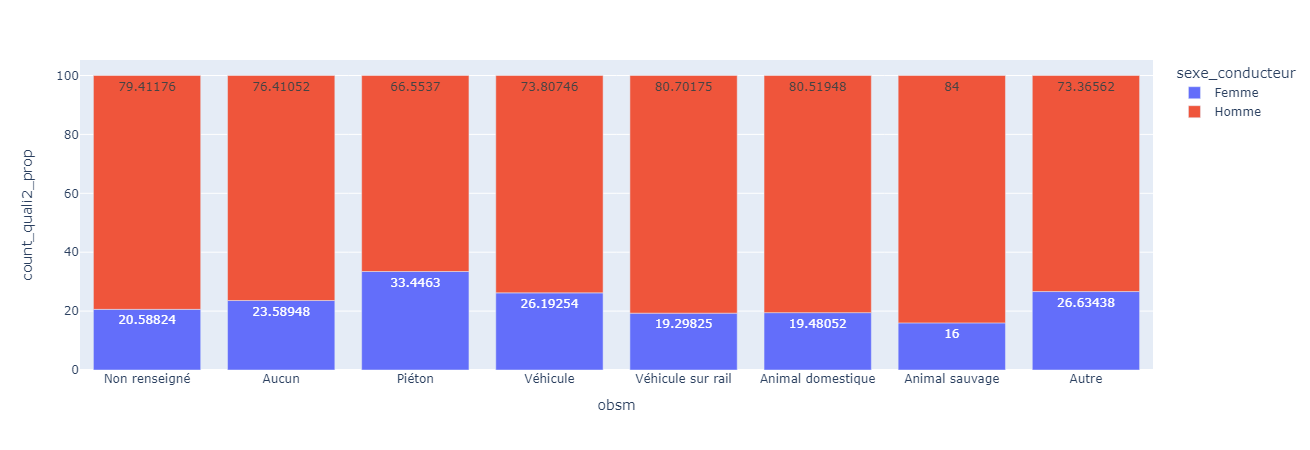
\includegraphics[width=7cm]{./img/bivar_sexe.png}
            \caption{Proportion femmes/hommes en fonction de la présence d'un obstacle dans l'accident}\label{fig:fig_sexe_bivar1}
        \end{subfigure}
        \hspace{0.2cm}
        \begin{subfigure}{7cm}
            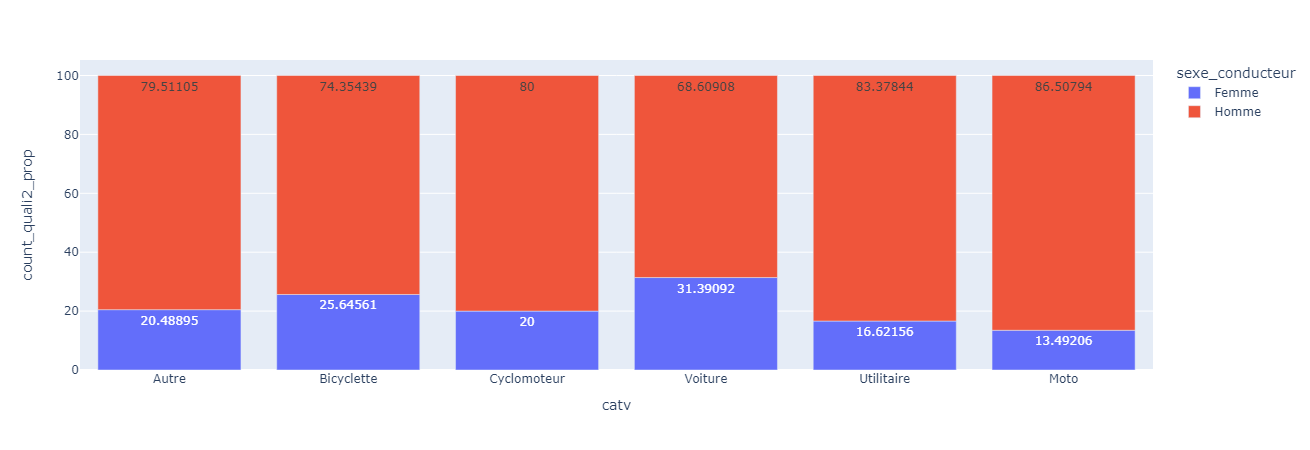
\includegraphics[width=7cm]{./img/bivar_sexe2.png}
        \caption{Proportion femmes/hommes en fonction de la catégorie du véhicule}\label{fig:fig_sexe_bivar2}
        \end{subfigure}
    \end{figure}
    \vspace{2cm}

    \subsubsection{Agglomération}
    L'attribut \textit{agg} indique si l'accident a eu lieu en agglomération ou hors agglomération. On retrouve 
    des corrélations plutôt logiques avec un certain nombre d'attributs comme par exemple une proportion d'accidents avec 
    piéton plus élevée en agglomération (figure \ref{fig:fig_agg_bivar1}). On peut également remarquer (figure \ref{fig:fig_agg_bivar2}) que la proportion 
    d'accidents en agglomération varie avec les conditions atmosphériques.
    Toutes ces corrélations peuvent nous indiquer que cet attribut va pouvoir contribuer à nos 
    prédictions.

    \begin{figure}[h]
        \centering
        \begin{subfigure}{7cm}
            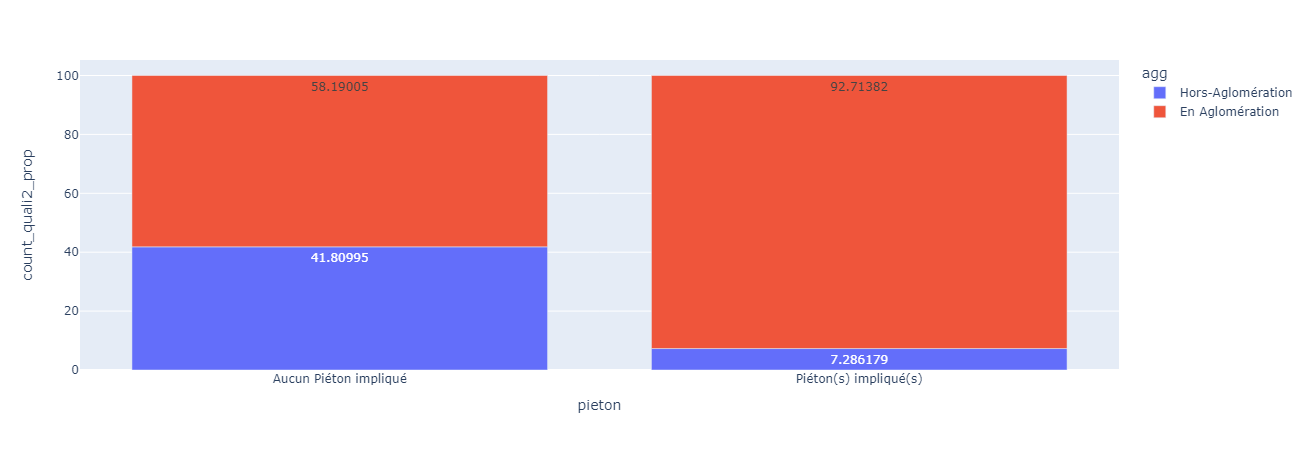
\includegraphics[width=7cm]{./img/bivar_agg.png}
            \caption{Proportion d'accidents en agglomération avec piéton et sans piéton}\label{fig:fig_agg_bivar1}
        \end{subfigure}
        \hspace{0.2cm}
        \begin{subfigure}{7cm}
            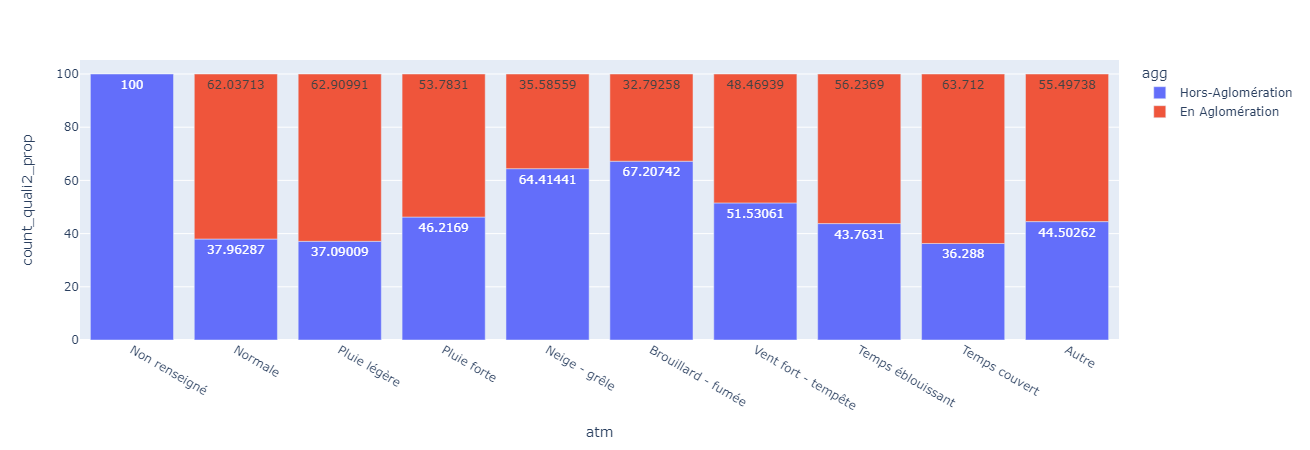
\includegraphics[width=7cm]{./img/bivar_agg2.png}
            \caption{Proportion d'accidents en agglomération en fonction des conditions atmosphériques}\label{fig:fig_agg_bivar2}
        \end{subfigure}
    \end{figure}
    
    \section{Apprentissage}
    
    \subsection{Split}
    Séparer nos données en deux ensembles demandait de tenir compte d'une spécificité. Nous nous plaçons du point de vue d'un véhicule. 
    Mais bien souvent, plusieurs véhicules sont impliqués dans un accident. Il nous a donc fallu adapter la division pour que les véhicules 
    d'un même accident soient dans le même ensemble. 
    
    Par ailleurs, nous avons constaté que ne pas adopter cette approche provoquait un surapprentissage lors du test. Typiquement, un trop grand 
    nombre de morts étaient correctement prédits.
    
    \subsection{Encodage One Hot}
    La base de données nous fournit pour la plupart des attributs des données qui peuvent être converties en entiers. 
    Par exemple, une catégorie de véhicule (\textit{catv}) est désignée par un chiffre. L'attribut reste cependant catégoriel. En pratique, 
    le seul attribut quantitatif qui nous reste est l'âge du conducteur. 
    Le reste est soit binaire, soit qualitatif. 
    
    Tous les attributs qualitatifs ont donc été transformés en OneHot. Initialement, nous souhaitions optimiser le nombre de colonnes en 
    réalisant les OneHot nous-mêmes. Par exemple, prenons "surf" (l'état de la surface de la route). Il est inutile de créer une colonne 
    pour "Non-renseigné", "Autre" ou "normale". Nous sommes uniquement intéressés par les états spécifiques de la route. 
    
    Cependant, cette approche posait des problèmes car elle empêchait la réalisation de l'audit. Nous avons donc utilisé la méthode 
    standard pour nos OneHot. 
    
    \subsection{Random Forest Classifier}
    Une fois les données prêtes, nous avons utilisé le classifieur d'arbres aléatoires pour obtenir un modèle. C'est le premier que nous 
    avons utilisé. En ce qui concerne les résultats, le score d'exactitude est de \textit{1} pour l'entraînement et de \textit{0.9014} pour le test.
        
    En ce qui concerne la matrice de confusion, on remarque que \textit{27687} véhicules ont été classés correctement en tant qu'accidents non létaux.
    Tandis que \textit{291} accidents mortels ont été correctement identifiés. Cependant, \textit{1413} accidents mortels ont été recensés à tort 
    comme étant non létaux et \textit{1648} véhicules ont subi le sort inverse. 
    
    \begin{figure}[h]
        \centering
        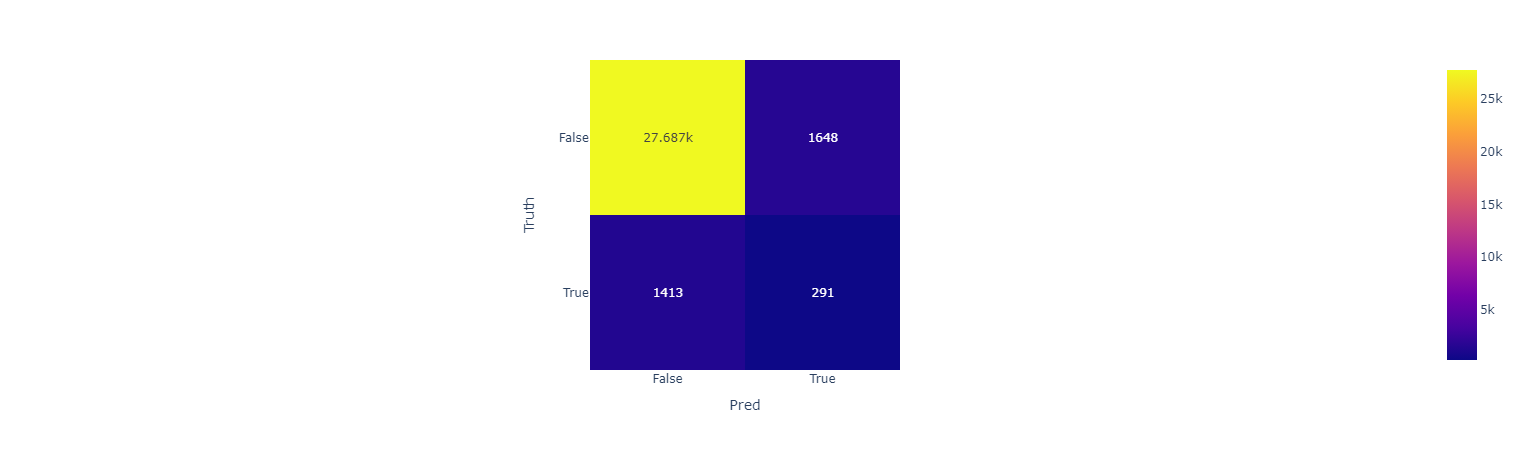
\includegraphics[width=\textwidth]{./img/matrice_confusion_tree.png}
        \caption{La matrice de confusion pour le classifieur d'arbres aléatoires}
    \end{figure}
    

    En résumé, on remarque que le modèle réussit très bien à classifier les accidents qui n'ont pas conduit à la mort de quelqu'un. Cependant, 
    il lui apparaît bien plus difficile de trouver les véhicules impliqués dans des accidents mortels. On peut attribuer ceci au fait que ces 
    accidents létaux ne représentent que \textit{5.38\%} des accidents répertoriés dans la base.

    \subsection{GaussianNB}
    Avancés dans le projet, nous avons voulu tester plusieurs classifieurs, tous ont donné des résultats différents, pour certains médiocres. 
    Mais nous avons trouvé un autre classifieur qui donnait des résultats intéressants : GaussianNB.
        
    Il ne maximise pas notre score de précision puisqu'il n'est que de \textit{0.8734} à l'entraînement et de \textit{0.8677} pour les tests. Ce qui 
    a toutefois retenu notre attention, c'est le nombre d'accidents létaux qu'il parvient à détecter : \textit{508}. Réduisant ainsi l'erreur des 
    accidents mortels recensés à tort comme étant non létaux à seulement \textit{1196}. Ceci entraîne malheureusement une perte de performances 
    pour ce qui est de la détection d'accidents non mortels comme on peut le voir ci-dessous.

    \begin{figure}[h]
        \centering
        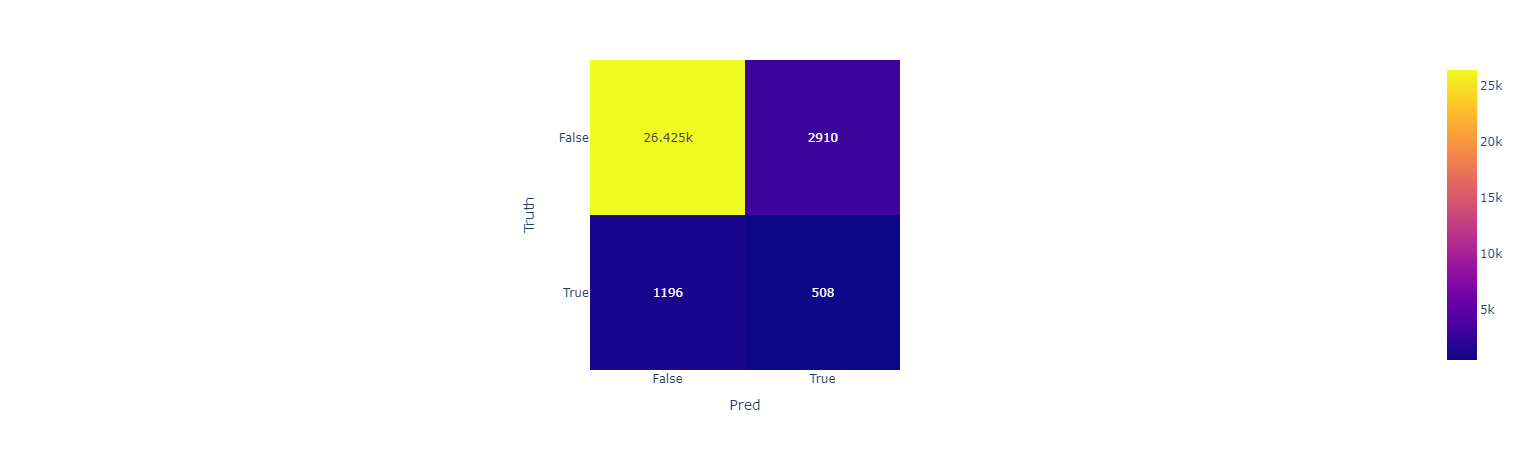
\includegraphics[width=\textwidth]{./img/matrice_confusion_gaussien.png}
        \caption{La matrice de confusion avec GaussianNB}
    \end{figure}

    Un autre avantage qui peut ressembler à un inconvénient au départ est que ce classifieur demande des nombres et non des OneHot. Or nous en 
    avons à foison. En dépit de ça, nos valeurs au départ sont en format numérique, rendant donc nos données compatibles avec cette approche.
    Ceci nous ouvre alors la possibilité de tester d'autres choses puisque le classifieur donne des probabilités et non des arbres. Au premier 
    rang desquels \textit{xplique}.
        
    Par souci de concision cependant, nous prendrons le modèle issu du \textit{random tree classifier} pour tous les audits qui vont suivre, 
    puisque c'est le premier avec lequel nous avons travaillé. On notera tout de même que lorsqu'on effectue ces audits avec \textit{GaussianNB}, 
    les résultats diffèrent en bien des points de ceux observés avec le \textit{random tree classifier}, preuve qu'ils ont une approche bien différente.

    \subsection{Base Rate}

    Nous avons voulu mesurer les résultats sur deux données potentiellement à protéger : le fait qu'un piéton soit impliqué dans 
    un accident et le sexe du conducteur. Voici les résultats :

    Sexe du conducteur 1 (un homme)

    Disparate Impact : 1.21767750298587 1.6331199049428085

    P-rule disparate Impact : 0.8212355057458954 0.6123249107266375

    Démographie Parité : 0.011747835864606336 0.02383701239031672

    Ce qui est flagrant ici, c'est qu'il existe une disparité dans la prédiction d'accidents mortels pour les hommes. Allant par ailleurs
    dans le sens de ce qu'indique Disparate Impact par la suite. Notons cependant que la disparité démographique existe mais est très
    faible.

    Piéton 1 (un piéton est impliqué)

    Disparate Impact : 1.0538191011165416 1.0968113720110815

    P-rule Disparate Impact : 0.9489294689576994 0.9117337999207913

    Démographie Parité : 0.003345154811069756 0.005266913173450724

    Pour ce qui est de l'implication d'un piéton dans un accident, on constate ici aussi une légère disparité, soulignant leur
    plus grande implication dans des accidents mortels. Ceci concorde encore une fois avec le \textit{disparate Impact}. Démographiquement, 
    le cas est similaire au sexe, puisqu'on constate une légère disparité en leur faveur, bien que cette fois la disparité soit plus
    faible encore.

    \section{Audit du modèle}

    \subsection{Génération des contrefactuels avec Dice}
    Dice nous a permis d'établir quels attributs influent sur la prédiction de notre modèle. Les résultats sont 
    cependant assez variables d'une exécution à l'autre. On peut tout de même retrouver lesquels sont fréquemment impliqués 
    dans le changement des exemples contrefactuels.
    Parmi eux, on peut noter que l'attribut \textit{âge} est souvent représenté. Le taux d'accidents (notamment mortels) étant plus 
    élevé chez les jeunes et les personnes âgées, cela paraît assez cohérent. L'attribut \textit{obsm} est également 
    souvent représenté dans les exemples contrefactuels.
    On a pu remarquer que l'attribut \textit{col} est peu représenté dans les résultats, contrairement à l'hypothèse que 
    nous avions pu faire lors de l'analyse.

    Enfin, les attributs \textit{dep} et \textit{sexe\_conducteur} sont également représentés. Ils pourraient être sources de biais, notamment 
    l'attribut \textit{dep} ; le modèle pourrait associer un département à une prédiction d'accident mortel.


    \subsection{BlackBoxAuditing}
    Les résultats que nous allons analyser sont issus du modèle généré par \textit{random tree classifier}.

    Tout d'abord, l'audit a porté sur les 24 features que nous avons conservés afin d'élaborer ce modèle. Ce qui marque avec 
    cet audit provient du sommaire. On y constate le rôle prédominant de l'âge pour l'accuracy score. À 0.84, ce dernier éclipse 
    tous les autres. Une explication pourrait venir de ce que nous avons constaté dans notre analyse univariée : il y a une 
    surreprésentation des jeunes de 20--21 ans dans ce set. Ceci est en réalité loin de surprendre puisqu'il s'aligne avec la 
    politique de prix pratiquée par les assureurs envers les jeunes conducteurs.

    Par la suite, on peut s'intéresser à l'évolution de l'accuracy en fonction du niveau de réparation appliqué à chaque 
    attribut :

    \begin{figure}[h]
        \centering
        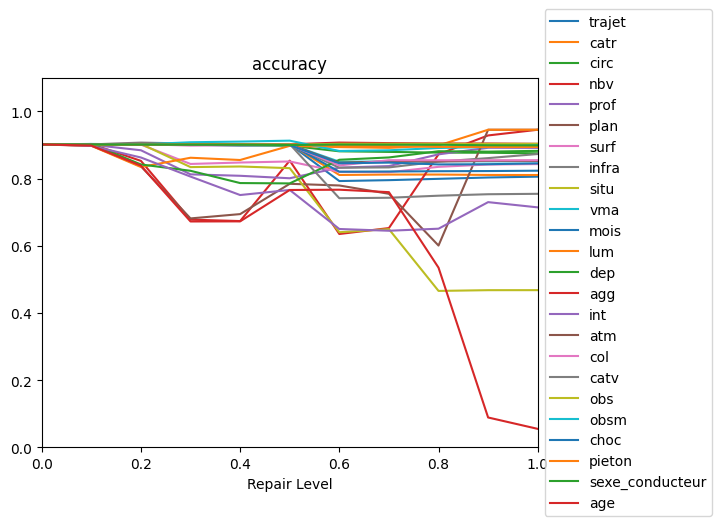
\includegraphics[width=10cm]{./img/accuracy.png}
        \caption{L'accuracy en fonction du niveau de réparation pour chaque attribut.}
    \end{figure}

    Ce qui est marquant ici est la disparité de réaction lors de l'application de mesures de réparations. On reconnaît les 
    attributs dont l'accuracy est au plus haut en regardant ceux qui s'effondrent le plus. En premier lieu, l'âge s'illustre
    à nouveau. À la lumière de ceci, il apparaît évident que le modèle discrimine fortement les véhicules en fonction de l'âge du 
    conducteur. Dans une moindre mesure, on constate la même chose pour \textit{situ}, qui fait référence à la localisation 
    géographique de l'accident. Ce qui paraît sensé, étant donné que certains lieux sont plus dangereux que d'autres. Enfin, 
    notons que le type d'intersection et la catégorie du véhicule sont également sources de discriminations de la part de notre 
    modèle. Encore une fois, cela semble cohérent.

    Toutefois, notons l'absence de quelques attributs notables tels que le nombre de voies, le sexe du conducteur (chose intéressante :
    ce n'est pas le cas avec GaussianNB), le type de collision, le type d'obstacle heurté ou encore le fait qu'un piéton soit impliqué.
    Pour ce qui est des piétons, cela peut paraître étonnant ; on peut émettre l'hypothèse que leur présence est souvent en ville là où 
    les vitesses sont basses entraînant donc moins de morts.

    Maintenant regardons l'équilibre du modèle à l'aide du BCR.

    \begin{figure}[h]
        \centering
        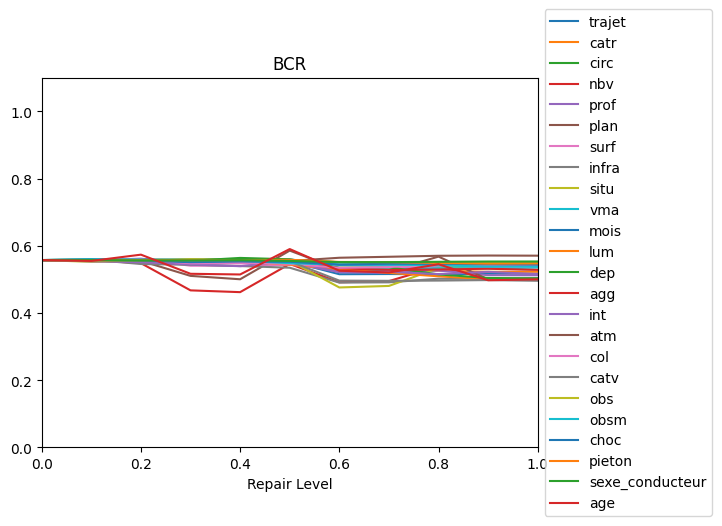
\includegraphics[width=10cm]{./img/BCR.png}
        \caption{Le BCR en fonction du niveau de réparation pour chaque attribut.}
    \end{figure}

    On remarque ici que les attributs sont plutôt centrés autour de \textit{0.5} et que la plupart reste rectiligne, mais que certains divergent
    quelque peu. Cet évasement est dû à des attributs déjà connus tels que \textit{âge} ou \textit{catv}. D'autres influent aussi mais ne s'étaient pas 
    illustrés précédemment, à l'image du nombre de voies, du profil de la route ainsi que de la luminosité. 

    Malgré cela, l'évasement assez faible laisse penser que le modèle est plutôt équilibré. De plus, comme mentionné précédemment 
    dans la section dédiée au split, nous avons pu tester le cas où on acceptait que des véhicules impliqués dans le même accident
    se retrouvent dans des ensembles différents (entraînement / test). Ce qu'il ressortait alors du BCR était un évasement beaucoup
    plus important et une origine située vers 0.68. Ce qui laisse à penser que cette version était bel et bien trop modelée sur le train
    set, l'équilibre était rompu.

    \subsection{Expliquer le modèle avec les valeurs de Shapley}
    Afin d'analyser la contribution des différents attributs dans notre modèle, nous avons 
    utilisé les valeurs de Shapley. Nous avons d'abord essayé de calculer la valeur exacte avec la fonction 
    \verb|ShapleyValues| du module \textit{ShapKit}. Cependant, le nombre d'attributs de notre dataset est trop 
    important et le calcul trop long.
    Il a donc fallu calculer une approximation de la valeur de Shapley avec la fonction \verb|MonteCarloShapley|.
    Nous devons cependant être prudents car le calcul de l'approximation nous 
    donne une tendance pour notre modèle mais certainement pas une valeur exacte. On peut le constater en changeant 
    le nombre d'itérations, ce qui produit un résultat différent.

    Avec \texttt{n\_iter=1000}, on obtient le diagramme en cascade de la figure \ref{fig:fig_shap}. Ce diagramme 
    nous montre, en partant d'un score référence de 1, quels attributs contribuent à obtenir un score de 0 (l'utilisation 
    d'un arbre de décision nous donne forcément une valeur binaire 0 ou 1, d'où le passage de 1 à 0).

    Les attributs qui contribuent le plus sont ici \textit{trajet}, \textit{agg}, \textit{circ}, \textit{mois} et 
    \textit{obsm}. On aurait pu ici s'attendre à une contribution plus importante de \textit{lum}, \textit{vma} ou 
    encore \textit{col} (qui ici a une contribution mineure).

    Une donnée intéressante ici est la valeur pour l'attribut \textit{sexe\_conducteur}. On nous donne une contribution 
    nulle de cet attribut, ce qui peut nous encourager dans l'idée que le sexe n'est pas un biais pour notre modèle. 
    Ce résultat étant une approximation, il est possible que la véritable valeur ne soit pas complètement nulle mais 
    du moins assez faible.

    Enfin, ce résultat nous montre que seule une petite partie des attributs contribue au résultat. On aurait 
    voulu une contribution un peu plus répartie entre les attributs car ici le changement d'une petite partie
    des attributs pourrait faire basculer le résultat. Or on sait bien que les 5 attributs qui contribuent ici le 
    plus ne permettent pas à eux seuls d'expliquer ce changement.

    \begin{figure}[h]
        \centering
        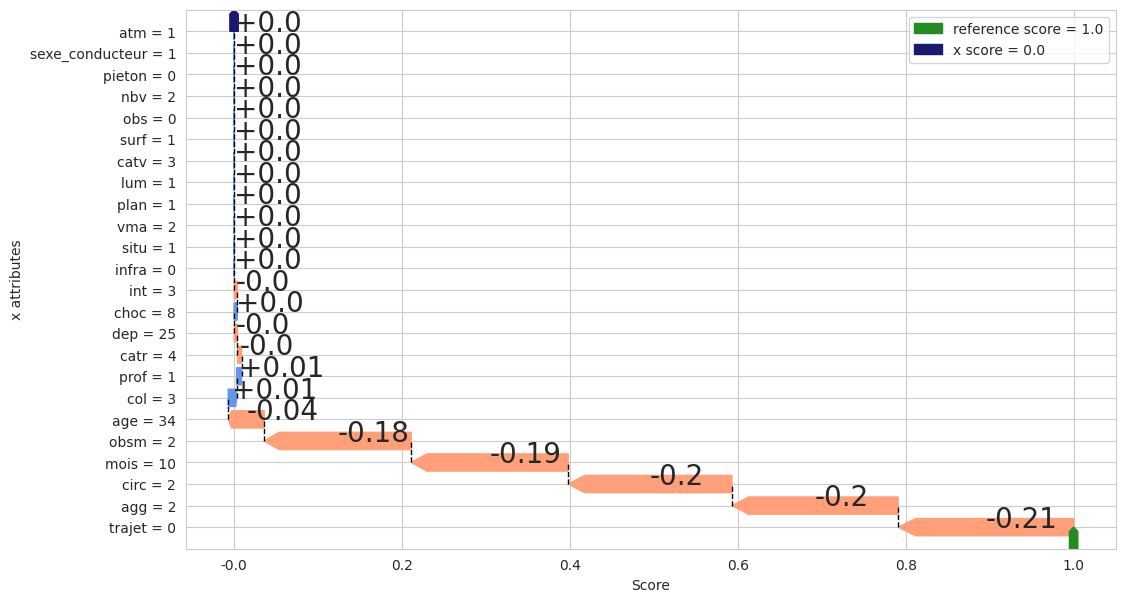
\includegraphics[width=\textwidth]{./img/shap1.png}
        \caption{Une approximation des valeurs de Shapley}
        \label{fig:fig_shap}
    \end{figure}

    \subsection{Expliquer le modèle avec Lime}
    Nous avons également utilisé \textit{Lime} afin d'avoir une idée des attributs qui contribuent
    le plus aux prédictions de notre modèle. On peut retrouver le code correspondant dans le fichier 
    \texttt{lime.ipynb}.

    Nous avons d'abord récupéré les indices des prédictions positives de notre modèle (avec quelles 
    entrées notre modèle prédit 1 ?). Ainsi, on a pu regarder dans les cas où les prédictions sont 0 
    et les cas où les prédictions sont 1.
    On peut remarquer qu'on trouve des variables similaires à celles trouvées avec les valeurs de 
    Shapley. On retrouve notamment assez fréquemment l'attribut \textit{agg}.
    Cependant, contrairement au résultat que pouvait nous donner \textit{ShapKit}, l'attribut \textit{mois} est 
    moins représenté. Les contributions sont également plus réparties entre les attributs.
    Enfin, il semble que comme nous avions pu l'observer avec les valeurs de Shapley, l'attribut 
    \textit{sexe\_conducteur} ait un faible impact sur la prédiction.

    \section{Conclusion}


    \newpage
    \appendix

    \section{Les données de notre dataset}\label{appendix:dataset}
    \begin{center}
        \begin{tabular}{ |c|p{9cm}| }
            \hline
            \textbf{Attribut} & \textbf{Description} \\
            \hline
            \textit{Num\_Acc} & Numéro d'identifiant de l'accident \\
            \textit{jour mois} & Jour de l'accident, mois de l'accident \\
            \textit{an} & Année de l'accident \\
            \textit{hrmn} & Heure et minutes de l'accident \\
            \textit{lum} & Conditions d'éclairage dans lesquelles l'accident s'est produit \\
            \textit{dep} & Code INSEE du département \\
            \textit{com} & Numéro de commune (code INSEE) \\
            \textit{agg} & Localisation en agglomération \\
            \textit{int} & Type d'intersection \\
            \textit{atm} & Conditions atmosphériques \\
            \textit{col} & Type de collision \\
            \textit{adr} & Adresse postale (pour les accidents en agglomération) \\
            \textit{lat} & Latitude \\
            \textit{long} & Longitude \\
            \textit{catr} & Catégorie de route \\
            \textit{voie} & Numéro de la route \\
            \textit{circ} & Régime de circulation \\
            \textit{nbv} & Nombre total de voies de circulation \\
            \textit{vosp} & Présence d'une voie réservée \\
            \textit{prof} & Profil en long de la route \\
            \textit{plan} & Tracé en plan de la route \\
            \textit{surf} & État de la surface de la route \\
            \textit{infra} & Présence d'aménagements ou d'infrastructures \\
            \textit{situ} & Situation géographique de l'accident \\
            \textit{vma} & Vitesses maximale autorisées \\
            \textit{id\_vehicule} & Identifiant du véhicule (clé étrangère) \\
            \textit{catv} & Catégorie du véhicule impliqué dans l'accident \\
            \textit{obs} & Type d'obstacle heurté \\
            \textit{obsm} & Type d'obstacle mobile heurté \\
            \textit{choc} & Point de choc initial \\
            \textit{manv} & Manœuvre principale avant l'accident \\
            \textit{catu} & Catégorie d'usager (conducteur, passager, piéton) \\
            \textit{grav} & Gravité de l'accident pour l'usager \\
            \textit{sexe} & Sexe du conducteur \\
            \textit{trajet} & Motif du déplacement au moment de l'accident \\
            \textit{mortal} & Indique si le véhicule est impliqué dans un accident mortel (calculé dans le notebook) \\
            \hline
        \end{tabular}
    \end{center}

\end{document}